%% LyX 2.0.2 created this file.  For more info, see http://www.lyx.org/.
%% Do not edit unless you really know what you are doing.
\documentclass[12pt,twoside,english]{report}
\usepackage{lmodern}
\renewcommand{\familydefault}{\rmdefault}
\usepackage[T1]{fontenc}
\usepackage[latin9]{inputenc}
\usepackage[a4paper]{geometry}
\geometry{verbose,tmargin=3.5cm,bmargin=3cm,lmargin=3.5cm,rmargin=3cm,footskip=1cm}
\usepackage{fancyhdr}
\pagestyle{fancy}
\setcounter{secnumdepth}{3}
\setcounter{tocdepth}{3}
\setlength{\parskip}{\medskipamount}
\setlength{\parindent}{0pt}
\usepackage{float}
\usepackage{graphicx}
\usepackage{setspace}
\usepackage{esint}
\usepackage[authoryear]{natbib}
\usepackage{nomencl}
% the following is useful when we have the old nomencl.sty package
\providecommand{\printnomenclature}{\printglossary}
\providecommand{\makenomenclature}{\makeglossary}
\makenomenclature
\setstretch{1.5}

\makeatletter
%%%%%%%%%%%%%%%%%%%%%%%%%%%%%% User specified LaTeX commands.
\usepackage{fancyhdr}
\pagestyle{fancy}
\fancyhead[RE]{\bfseries \nouppercase\leftmark}
\fancyhead[LO]{\bfseries \nouppercase \rightmark}

\renewcommand{\chaptermark}[1]{%
\markboth{\chaptername 
\ \thechapter\ }{}}

 
\fancyhead[LE,RO]{\bfseries\thepage}
\fancyfoot{}
\raggedbottom
\setlength{\parindent}{8mm}

\makeatother

\usepackage{babel}
\begin{document}

\chapter{The Electricity Model\label{chap:The-Energy-Model}}

\newpage{}


\section*{Summary}

\noindent This chapter presents the development of the electricity
model utilised in Part 2 of this thesis. The components of the model,
some of the costs used and the locations from within the ACCESS-A
model grid utilised are outlined. A transmission cost is also presented,
and the chapter concludes by explaining how the individual components
are combined and what the specific combinations imply about the preferred
solutions to the electricity system configuration.

\noindent \newpage{}


\section{Introduction}

The electricity model utilised in this thesis is part of a collaborative
project that involves the Melbourne Energy Institute (University of
Melbourne) and the Australian Energy Research Institute at the University
of New South Wales. The aim of the model as a whole is to provide
a least cost combination of technologies (primarily renewable technologies)
that satisfy a particular target (carbon emission reduction, renewable
electricity percentage, reliability, etc.). The optimised problems
in this thesis are, however, intentionally less focused on the feasibility
of implementing the solutions, in order to maintain the focus on the
regional influential meteorological factors. 

The electricity model in this thesis balances the output of each given
technology, combines the costs involved into a single dollar amount
and then informs an optimisation algorithm of the total cost of each
iteration of the solution space. The electricity model ensures that
demand is met by each mixture of technologies and the total cost will
vary based on the amount that each resource is utilised (a similar
process was used in \citet{Huva2012} and Fig. \ref{fig:Huva-etal-2012-Model-Output}
illustrates how the resources can be combined). In the case of the
current study the cost function to be minimised is a combination of
costs assigned to each of the available technologies (in this case
onshore wind, large-scale concentrating solar, pumped hydro storage
and gas fired back-up). The costs for each technology define the order
in which the technologies are favoured---the dispatch order. For all
simulations examined in this thesis the effective dispatch order is
renewables (wind and solar), followed by hydro and then gas. 
\begin{figure}[H]
\noindent \begin{centering}
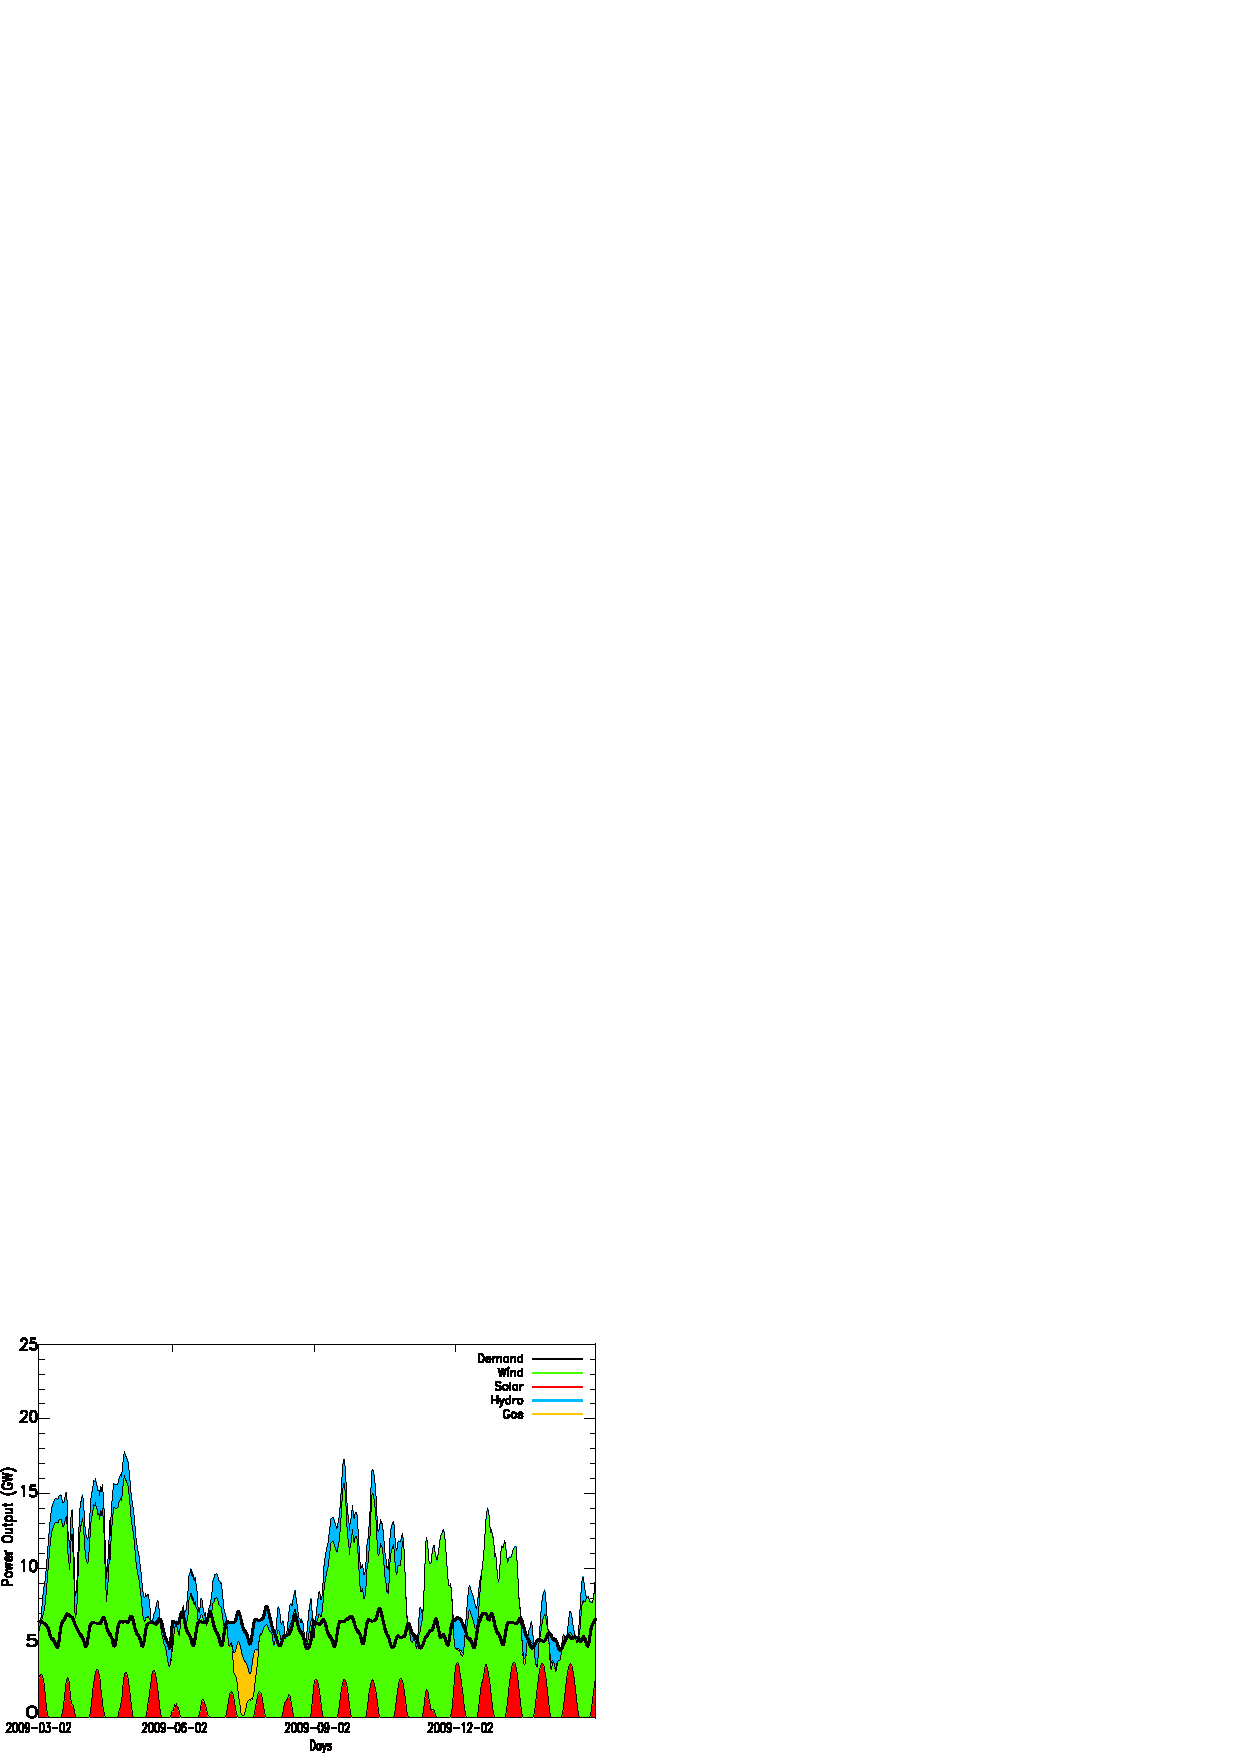
\includegraphics{Figures/CoV_output_miss_poly}
\par\end{centering}

\caption{Example electricity model output. The curves are additive such that
the wind output (green) is built upon the solar output (red) with
gas (orange) and then hydro (blue) to follow. Hydro output below the
demand (black) curve indicates release of pumped storage, while above
the curve indicates pumping up hill. Figure originally presented in
\citet{Huva2012}.\label{fig:Huva-etal-2012-Model-Output}}
\end{figure}


The optimisation technique used in the electricity model is a Genetic
Algorithm (GA). The GA is one possible tool for optimisation of complex
(non-linear) problems. The specific implementation of the GA in the
thesis is outlined in \citet{Rayner2003}. The GA is a population-based
meta-heuristic that, as described earlier, will have a population
of parameter combinations evolve/change over successive iterations
of the solution space. In general terms the GA behaves much like a
biological system on Earth. The evolution of the population is based
on values of the cost function (fitness) and user-defined control
parameters that govern rates of breeding, mutating, culling and cloning.
Breeding involves making new members of the population from pairwise
combinations of current members, mutating involves randomly changing
elements of population members and culling involves removing members
of the population, which are then filled-in by cloning remaining members
of the population (\citet{Rayner2003}). The propagation of fitter
members over generations is aided by selection of less fit members
at the cull stage (\citet{Rayner2003}).

Compared to other advanced techniques \citet{Fadaee2012} found the
GA, along with the Particle Swarm Optimisation \nomenclature{PSO}{Particle Swarm Optimisation}(PSO)
technique, to be a useful and promising technique for optimisation
of hybrid renewable energy based systems. The PSO technique searches
the solution space by sending out 'particles', which change their
position over time based on information gained from neighbouring particles
and by incorporating some memory of where it has been. \citet{Angeline1998}
compared the GA and PSO techniques and found both to perform well.
The PSO was seen to equilibrate on near optima more quickly than the
GA, but was also less able to explore the solution space any further
due to a lack of adaptability. The GA was seen to be more adaptive
in these final stages of searching, despite taking more time to get
to that point (\citet{Angeline1998}). An advantage of the population-based
algorithms is the ability to trade-off between many parameters and
analyse several near-optimal solutions \citet{Banos2011}. This flexibility
reduces the likelihood of the algorithm becoming stuck in local minima.
However, depending on the problem at hand it is possible for their
to exist many near optimal solutions that contain vastly different
parameters but have similar cost function values. As stated earlier,
the flexibility of a population-based technique comes at the price
of ambiguity.

As was mentioned in the previous chapter it was not seen as possible
to utilise one of the many pre-built electricity/energy models. Further,
with a lack of specific evidence to suggest that one particular optimisation
technique will be best suited for the problem at hand it was decided
to utilise the GA. The following sections describe the components
of the electricity model, as well as a pre-optimisation site selection
process. The optimisation problem is more amenable to optimisation
if it is given to the GA in a succinct version. In the site selection
process a sub-selection of all available locations is made. A completely
unrestricted optimisation would involve searching the solution-space
in regions that included unrealistic solutions. Thus, similar to the
user-defined costs, the site selection process is part of the concept
that the user has some knowledge of the nature of the problem before
undertaking the optimisation. 


\section{Cost Function and Components\label{sec:Optim-Cost-Function}}

In this thesis the cost function is defined as being made up of costs
from the building and maintenance of renewable electricity resources,
as well as costs associated with back-up electricity supply, and other
costs involved in the maintenance of the electricity system. The goal
of the GA is to minimise these costs, and in doing so provide information
regarding the optimal combination of wind and solar to meet the electrical
demand of Australia. Thus, in the optimisation process the electricity
model is given not only the value of the cost function but also the
installed capacity of the wind and solar resources. At each iteration
of the optimisation process the GA determines whether or not it would
be more/less cost effective to install more/less wind or solar resources
at each available site selected from the ACCESS-A model grid. As will
become more evident later on in the thesis, and based on the costs
used in each scenario, the aim of electricity model could be thought
of as minimising gas usage. Gas has the highest costs in all scenarios
examined in this thesis and thus it is attractive in a cost-cutting
sense for the electricity model to minimise gas usage wherever possible.
The details of the cost function components are outlined in the sections
below.


\subsection{Renewable electricity costs\label{sub:Renewable-energy-costs}}

The costs for the wind and solar resources in this thesis were determined
based on the idea that each wind/solar site has an initial installation
cost and then costs associated with building and installing the required
amount of wind/solar technology. Further to this, and based on an
economy of scale, the installation of each new wind turbine or large-scale
solar unit should increment such that the increments get progressively
smaller and asymptote towards just the manufacturing cost. The asymptotic
behaviour of such a total site cost vs. number of units relationship
is theoretically the same for both technologies, however the rate
of change of the asymptote gradient will be different for each technology.
The gradient behaviour of the relationship between cost and number
of installations can be described by the following relationship: 

\begin{equation}
gradient\,\, behaviour\sim\frac{a}{b}\frac{\sqrt{a+(bn)^{2}}}{n}\label{eq:Gradient-Behaviour}
\end{equation}


It is clear from Eq. \ref{eq:Gradient-Behaviour} that the gradient
behaviour for an economy of scale follows this relationship because
taking the limit of Eq. \ref{eq:Gradient-Behaviour} with respect
to $n$ tends towards $a$ (the capex, below); where the rate at which
this tendency occurs is controlled by the parameter $b$. Once the
gradient behaviour was formed it was then possible to integrate the
relationship and obtain a formula for the total system cost per new
installation ($n$). The solution to this integration is shown in
Eq. \ref{eq:Cost-Function-Solution} and an example of the function\textquoteright{}s
behaviour with increasing $n$ is shown in Fig. \ref{fig:Cost-Function-Example}---this
is concordant with the study by \citet{Elliston2013} who suggested
that for a study using a GA penalties are best introduced gradually
than by a step function. 

\begin{equation}
\frac{a}{b}\int\frac{\sqrt{a+(bn)^{2}}}{n}\,\, dn=\frac{a[\sqrt{a+(bn)^{2}+\sqrt{a}ln(\frac{n}{a+\sqrt{a(a+(bn)^{2}}})}]}{b}\label{eq:Cost-Function-Solution}
\end{equation}


where, $a=capex$ (the capital expenditure costs), $b=\alpha capex^{3}-\beta capex^{2}+\gamma capex+c$
and $\alpha,\beta,\gamma$ and $c$ are tuned constants.

The tuned constants in Eq. \ref{eq:Cost-Function-Solution} were iteratively
determined such that the gradient of wind cost versus number of turbines
approached values very close to the manufacturing costs of a turbine
for wind at approximately 15 Turbines (Cowling P., Pers. Comm., Jan
23 2013) and for solar at approximately five large-scale concentrating
units. While such asymptotic behaviour might weaken at much larger
numbers of turbines/solar stations (for instance, the cost of additional
infrastructure including new substations at large numbers might alter
the relationship), it is a useful relationship for the purposes of
this thesis. Without a large initial cost (cost for the first turbine/solar
station) and high incremental costs for low numbers of turbines/solar
stations it could be cost effective to install large amounts of small
wind/solar installations. In reality though, this would not be cost
effective given the relatively high cost of infrastructure for a new
installation compared to the cost of an individual turbine/solar station.
To aid the GA in finding solutions with more consolidated infrastructure
it was found that the relationship seen in Fig. \ref{fig:Cost-Function-Example}
and described by Eq. \ref{eq:Cost-Function-Solution} was necessary.
\begin{figure}[H]
\noindent \begin{centering}
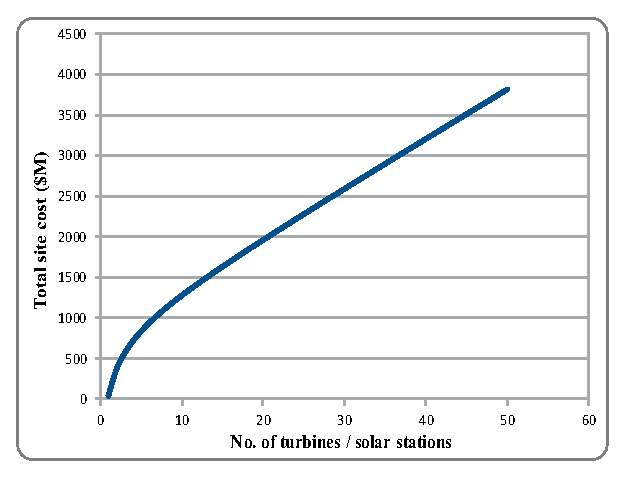
\includegraphics{Figures/Cost_fnct_exmpl}
\par\end{centering}

\caption{Example of the solution to Eq. \ref{eq:Cost-Function-Solution}. \label{fig:Cost-Function-Example}}
\end{figure}



\subsection{Hydro Model\label{sub:Hydro-Model-Description}}

The first form of back-up electricity supply in the electricity model
was via pumped hydro power. The hydro model in its simplest form utilises
excess electricity from the renewable resources and pumps it uphill
for later use. By pumping the water uphill the potential energy of
the system is increased. If, in subsequent hours, the renewable resources
cannot supply enough electricity to meet demand the hydro model will
release the water downhill. By releasing the water downhill the stored
potential energy is converted to kinetic energy. Electrical energy
is then produced from the spinning of large turbines immersed in the
downhill pipes. At each iteration of the optimisation of the electricity
model the hydro model is deployed in a post-facto manner. For each
iteration of the optimisation a time series of output from the selected
wind and solar installations is produced and thus a time series of
the difference between renewable output and demand is also formed. 

The hydro model takes the difference time series and uses the moments
of excess to pump water uphill---up to a pre-determined cap and with
a pre-determined maximum rate. The hydro model, which is also given
a pre-determined initial storage level then assesses each point in
time in the two-years of simulation and determines whether or not
water needs to be pumped, released, if no action is needed or if no
action is possible due to capacity constraints/storage levels. Thus,
a time series of hydro electrical output or storage of excess (negative
output) is also determined. The cost of the hydro system needed is
then a multiple of the maximum capacity needed and pre-determined
capital cost in the units of \$M/MW. It should also be noted that
the round-trip efficiency of the pumping system utilised in this thesis
was 0.8. This efficiency is in accordance with that used by \citet{Elliston2012}
in their simulation of 100\% RE for the NEM.


\subsection{Gas back-up Model \label{sub:Gas-Model-Description}}

The final electricity source available in the electricity model is
the gas-fired back-up system. The gas model is intentionally last
in the dispatch order of resources due to the nature of this study,
which is focused on determining the likelihood of Australia relying
heavily on renewable resources in the future. The gas model is assumed
to have the ability to be fired instantaneously to meet any remaining
demand that cannot be met by the combination of wind, solar and hydro.
The cost of the gas system is described by Eq. \ref{eq:Gas-Cost-Formula}.
Where, $cost_{var}$ is the sum of the gas output (MW) multiplied
by a combination of pre-defined fuel and carbon prices, $cost_{var\_mult}$
is defined as a factor of roughly 1,000 that is implemented in order
to reflect the true fuel cost of a gas-fired plant over its lifetime
(\textasciitilde{}20 years, rather than the two years being simulated
in this thesis), the $max\_cap$ is the maximum installed capacity
needed and the $capex$ is the pre-determined capital cost of installing
the gas plant at the required size (units of \$M/MW).

\begin{equation}
Gas\,\, Cost=cost_{var}\cdot cost_{var\_mult}+capex\cdot max\_cap\label{eq:Gas-Cost-Formula}
\end{equation}



\subsection{Transmission Cost\label{sub:Transmission-Cost-Description}}

A transmission cost is utilised in parts of this study in order to
reflect the higher cost of connecting remote locations to the existing
electrical infrastructure. There is, however, no transmission model
that simulates power flow across Australia incorporated in this thesis.
It was assumed the incorporation of such a model in the current study
would likely distract from the study of the covariance of the wind
and solar resources. The addition of power flow would also be more
of an engineering question than a resource availability question (for
instance power flow would introduce restrictions to do with nodes
in the network and not the quality of the resource on its own). Instead,
the transmission model utilised in this thesis is simply a capital
cost that relates to the distance of each wind/solar site to the nearest
capital city. Based on population size and for the sake of geographical
diversity the capital cities used were Adelaide, Melbourne, Sydney,
Brisbane and Townsville. The capital cost utilised was in accordance
with \citet{Humpert2012} who suggested that high-voltage direct current
cabling costs approximately \$1M/km to build. High voltage DC transmission
lines are the type of cabling commonly used to connect remote locations
(which makes up the majority of locations in Figs. \ref{fig:Sites_Wind11_Dsr21}a
and \ref{fig:Sites_Wind11_Dsr21}b). In this way the transmission
cost penalises remote locations with an additional higher cost of
installation.


\subsection{Cost Function Evaluation\label{sub:Cost-Function-Evaluation}}

The total cost of the whole system at each iteration of the electricity
model is a combination of installation, connection, manufacturing
and fuel costs, as is applicable to each technology. The total cost,
to be minimised by the model, is therefore also in dollars. However,
these costs (potentially different in each simulation, and outlined
later) are not necessarily intended to be realistic. In terms of the
optimisation by the GA the most important consideration is whether
or not the costs are relatively in proportion and achieve the final
goal of also maximising the use of renewable electricity in the system.
What is important for the optimiser is the effect on the total cost
when additional capacity is installed or removed. The relative change
in system cost and the advantage/disadvantage in adding/removing capacity
is what determines the competitiveness of such an alternative solution,
rather than the total cost of the previous iteration.


\section{Site Selection Process\label{sec:Site-Selection-Process}}

This section describes the site selection process for the wind and
solar technologies. Power flow is not modelled in this thesis and
as such the hydroelectric and gas-fired power plants have no location
in space. Rather, the back-up resources are dispatched instantaneously
to the amount that is needed at the time for across the network (the
so-called 'copper plate' model). In terms of the wind and solar siting
it is sensible for a study that involves large meteorological data
sets to be mindful of limitations, both in a time-management and computation
sense. In particular, the optimisation in this thesis of all continental
locations within the ACCESS-A domain would be infeasible. It is also
not necessary to optimise all locations that contain meteorological
data. As seen in Part 1 there are decorrelation lengths that exist
in the atmosphere for most fields (in particular the wind field, but
also the solar field), which dictate that adjacent locations have
significantly similar time series. Using the knowledge of such a decorrelation
length in the wind field it was determined that a sub-selection of
available locations be utilised for the optimisation in Part 2. A
minimum spacing between available locations in the wind field was
determined to be 11 grid points, or roughly 120km. This minimum spacing
is considerably shorter than the decorrelation length scale of roughly
1,300km determined in Part 1. It was deemed possible to utilise a
shorter minimum spacing because the computational resources permitted
the utilisation of the 'extra' grid-points, even if no significantly
different information was gained by doing so. 

In terms of the Downward Shortwave Radiation (DSR) field, however,
no such decorrelation length scale was found in Part 1. This is not
to suggest that one location would be a diverse-enough selection for
all of Australia---this would mostly likely be unworkable in reality.
Instead, and even though two locations in the DSR field that are very
close might not provide any new information, the limitation on the
amount of DSR locations to include was purely computational. As such,
it was determined that the minimum separation of available DSR locations
would be 21 grid points---or roughly 250km. 

Following the determination of the minimum separation distances in
the DSR and wind fields the next step in the site selection process
was the elimination of potential locations that were unavailable due
to existing land-usages. Knowledge of the existing land-usages across
Australia was sourced from the Geoscience Australia GIS data-base.
Land-usage that included national parks and urban areas were combined
and mapped onto the ACCESS-A grid. These unavailable locations were
then utilised in the site selection process such that a regular grid
of locations was formed. The regular grid included the minimum separation
distance and did not include an unavailable site---in accordance with
a similar process outlined in (\citealp{AEMO2013}). Fig \ref{fig:Sites_Wind11_Dsr21}
shows this regular grid of available and separated locations for the
wind (Fig. \ref{fig:Sites_Wind11_Dsr21}a) and solar fields (Fig.
\ref{fig:Sites_Wind11_Dsr21}b). The total number of locations utilised
for the wind field (Fig. \ref{fig:Sites_Wind11_Dsr21}a) was 212 and
for the solar field (Fig. \ref{fig:Sites_Wind11_Dsr21}b) 58. These
locations will then be used in the next section as part of the optimisation.
\begin{figure}[H]
\noindent \begin{centering}
\includegraphics{Figures/RegGrid_ACCESS_wind_11_dsr_21_point_exclusion_with_natparks-capad}
\par\end{centering}

\caption{Locations from within the ACCESS-A grid chosen for input into the
electricity model. Red dots in a) represent the wind sites and in
b) represent the solar sites.\label{fig:Sites_Wind11_Dsr21}}
\end{figure}



\section{Conclusion\label{sec:Energy-Model-Conclusion}}

This chapter presented the electricity model used in Part 2 of the
current study, its components and also the site selection process
and transmission cost used to narrow the search for viable RE locations
around Australia. In combination, the cost function components (the
individual resource models) and the sites selected form the degrees
of freedom by which the model as a whole is able to move and explore
the solution space. Based on the specific GA configurations outlined
later, the GA alters the amount and location of RE resources in order
to find cost minimised solutions. In the next chapter simulations
of the whole of Australia and then just the NEM region are presented
and analysed for what they reveal regarding the covariance of wind
and solar across Australia. 
\end{document}
